\documentclass{lecturesimple}

\newcommand{\DateOfShow}{HT2023}
\newcommand{\Startdag}{måndag}
\newcommand{\KursStartTidDod}{tisdag kl 15 i E:A}
\newcommand{\KursStartTidPgk}{måndag kl 13 i E:A}
\newcommand{\BokpaketBilligt}{485}
\newcommand{\BokpaketDyrt}{810}
\newcommand{\Swish}{123 170 4584}

\title[Kort presentation av pgk \& dod, \DateOfShow]{\textbf{EDAA45} Programmering, grundkurs (pgk) \\ + \\ \textbf{EDAA60} Datorer \& datoranvändning (dod)}
\author{\href{http://cs.lth.se/bjorn-regnell}{Björn Regnell}, \href{https://cs.lth.se/nordahl-mattias/}{Mattias Nordahl}}
\institute{\href{http://cs.lth.se}{Datavetenskap}, LTH}
\date{\DateOfShow}

\begin{document}

\frame{\titlepage}

\begin{frame}\frametitle{Svensk skoldator på 1980-talet: ABC80, 64kB RAM}
  \begin{center}
      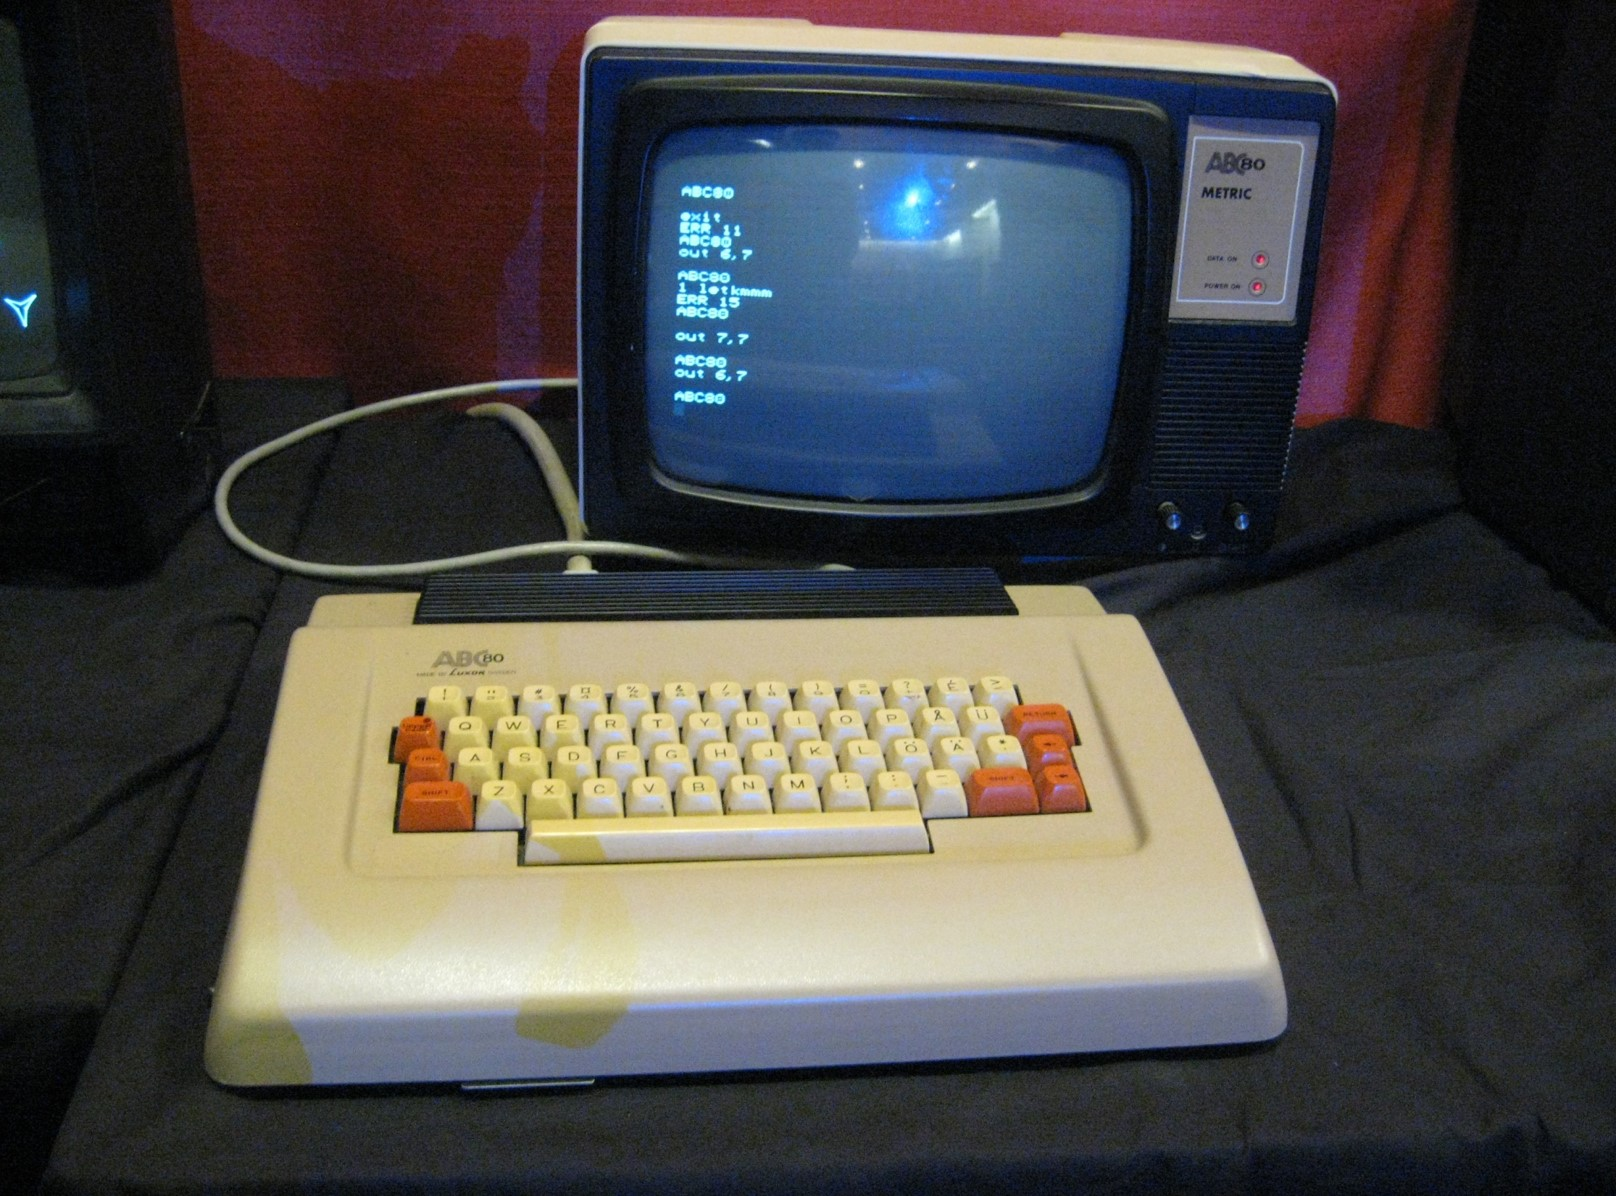
\includegraphics[width=1.0\textwidth]{../img/abc80}
  \end{center}
  \end{frame}
  
  
  \begin{frame}\frametitle{Stordator 1986: IBM 3090, % 69MHz,
      128MB RAM}
  \begin{center}
      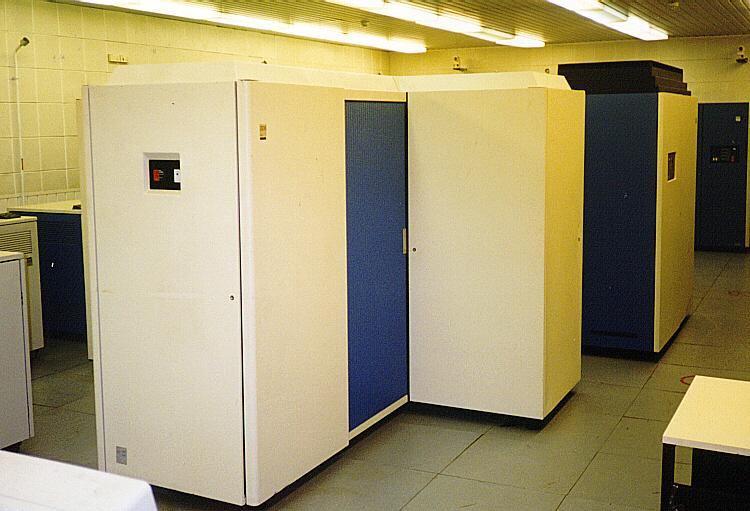
\includegraphics[width=1.0\textwidth]{../img/ibm3090.jpg}
  %     % http://hampage.hu/oldiron/e_ibms.html
    
      {\fontsize{5}{5}\selectfont\color{gray}
      Foto: hampage.hu/oldiron
    }
  \end{center}
  \end{frame}
    
  \begin{frame}\frametitle{Serverhall 2016: 28 000 kvm, 1 TWh/år, \\tusentals datorer, var och en minst 32GB RAM}
    \begin{center}
      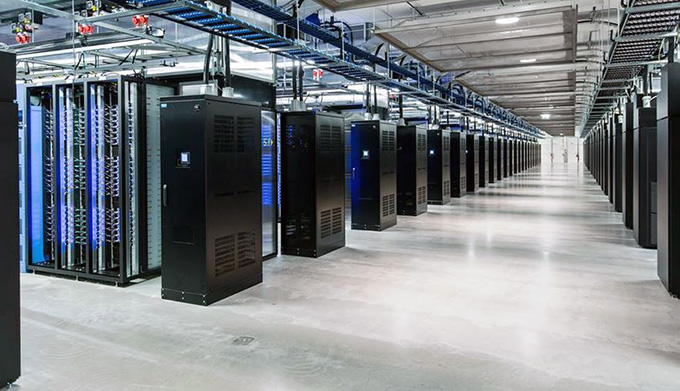
\includegraphics[width=1.05\textwidth]{../img/lulea-datacenter.jpg}
      % https://www.nextplatform.com/2016/03/10/inside-the-systems-that-drive-facebook/
      % https://nyadagbladet.se/wp-content/uploads/2013/06/lulea-datacenter.jpg
      % http://gamla.hbl.fi/nyheter/2013-07-06/471016/facebook-placerade-serverhallar-i-lulea
    
      {\fontsize{5}{5}\selectfont\color{gray}
    Foto: Facebook
    }
    \end{center}
  \end{frame}
  


\begin{Slide}{Digitaliseringens 2 största utmaningar}
  \begin{itemize}\Large
    \item Hantera ständiga \Alert{komplexitetsökningen}
    \item Åtgärda allt svårare \Alert{kompetensbristen} 
  \end{itemize}  
\end{Slide}

\SlideImg{Välutbildade inom IT är oerhört eftertraktade}{../img/kompetensbrist}


\frame{\frametitle{En kurskombo som startar på \Startdag}
Lägger grunden för alla kommande kurser i datavetenskap: \vspace{1em}
\begin{itemize}
  \item \Alert{Programmering, grundkurs} (pgk), 7.5 hp, 16 veckor
  \begin{itemize}
    \item[] En grundlig genomgång av programmering \Emph{från början} \\ med stora möjligheter till \Emph{fördjupning} som du själv väljer
  \end{itemize}
  \vspace{1em}
  \item \Alert{Datorer och datoranvändning} (dod), 3 hp, 3 veckor
  \begin{itemize}
    \item[] Inblick i hur datorer fungerar och verktygen vi använder
  \end{itemize}
\end{itemize}
}


\begin{Slide}{Tips för framgång i programmeringsstudier}
  \begin{itemize}
    \item Motivation att gå på djupet
    \item Hårt arbete
    \item Effektiv studieteknik
    \item Uppmuntrande socialt sammanhang
  \end{itemize}  
\end{Slide}

\frame{\frametitle{Vad ska du lära dig?}
%Att skapa koden som styr världen...
%\includegraphics[width=1.2\textwidth, height=1.5cm]{img/code-wide}
\begin{multicols}{2}
\begin{itemize}\Size{9pt}
\item \textbf{Programmering, grundkurs}
\begin{itemize}\Size{8pt}
\item Tänka i \Emph{abstraktioner}
\item Använda \Emph{datastrukturer}
\item Implementera \Emph{algoritmer}
\item Begrepp som lägger \Alert{grunden} för resten av din utbildning
\item Språk: \Emph{Scala}
\end{itemize}
\columnbreak
\item \textbf{Datorer \& datoranvändning}
\begin{itemize}\Size{8pt}
%\item Lågnivåprogrammering
%\item Datarepresentation
\item Terminalkommando i \Emph{Linux}
\item Skriva \& typsätta i \Emph{\LaTeX}
\item Versionhantering med \Emph{Git} 
\item Koddelning med \Emph{Github} 
%\item Beräkningar i Matlab
\end{itemize}
\end{itemize}
\end{multicols}
\vspace{2em}
\flushright\scriptsize Denna presentation i \LaTeX\ på GitHub:
\\{\tiny\url{https://github.com/lunduniversity/introprog/blob/master/slides/info-week00.tex}}
}

%%%
\frame{\frametitle{Hur ska du lära dig?}
\begin{itemize}
\item Genom praktiskt eget arbete: Lära genom att göra!
\begin{itemize}
\item Övningar
\item Laborationer
\item Projekt
\end{itemize}
\item Genom studier av viktiga begrepp: Skapa förståelse på djupet och lägga bred grund för din fortsatta utbildning
\item Genom samarbete med dina kurskamrater
\end{itemize}
}

%%%
% \frame{\frametitle{Kurslitteratur}
% \footnotesize
% \begin{columns}
% \begin{column}{0.65\textwidth}
% {\Size{16pt}pgk:}
% \begin{itemize}
% \item 2 st kompendier 358+360 sidor \\ Säljs till självkostnadspris på institutionen. \\ Beställ bokpaket om du inte redan gjort det här \Alert{senast idag kl 12} för mängdrabatt: \url{http://cs.lth.se/pgk/bokpaket}
% \end{itemize}
% \vspace{1em}
% {\Size{16pt}dod:}
% \begin{itemize}
% \item Kursmaterial delas ut på första föreläsningen.
% \end{itemize}
% \end{column}
% \begin{column}{0.35\textwidth}
% \centering
\includegraphics[width=0.99\textwidth]{../img/compendium-front-page-2019.png}
% \end{column}
% \end{columns}
% }



\SlideImg{Stor spridning i förkunskaper}{../img/survey-2023}

\frame[plain]{\frametitle{Beställ bokpaket!}
Bokpaketet är \Emph{fantastiskt!}\\~\\
\url{http://cs.lth.se/pgk/bokpaket}\\~\\
\Alert{Om du inte fyllt i den gör det nu!}\\ (Om du svarat ''Nej'' kan du ångrar dig och efterbeställa.)
}



\begin{Slide}{Bokpaket}
  \begin{itemize}
  \item C+D får hämta ut bokpaket mot uppvisande av Swish-transaktion via faddrar senare i veckan:
  \item[] *** Swishnummer: \Alert{\Swish}
  \item[] *** Ange meddelande: \textbf{pgk DittFörnamn DittEfternamn}
  \item[] *** Belopp: \Emph{\BokpaketBilligt} kr 
  \item[] Denna info finns också i Canvas.
  \item De som missat fadderutdelningen, samt W:are, hämtar ut efter överenskommelse med \url{birger.swahn@cs.lth.se} mot uppvisande av Swish-transaktion enl ovan.
  \item De som beställer innan kl 15 idag får paketpriset \BokpaketBilligt kr, sedan kostar enstaka tryck \Alert{\BokpaketDyrt} kr. \Emph{Efterbeställning} är möjlig från idag via Canvas. 
  \end{itemize}
\end{Slide}


\frame{\frametitle{Välkommen till kursstart!}
Kom i god tid till första föreläsningen enl. \url{https://cs.lth.se/pgk/schema/timeedit/}
\begin{itemize}
\item  pgk: \KursStartTidPgk
\item  dod: \KursStartTidDod 

%\item[] 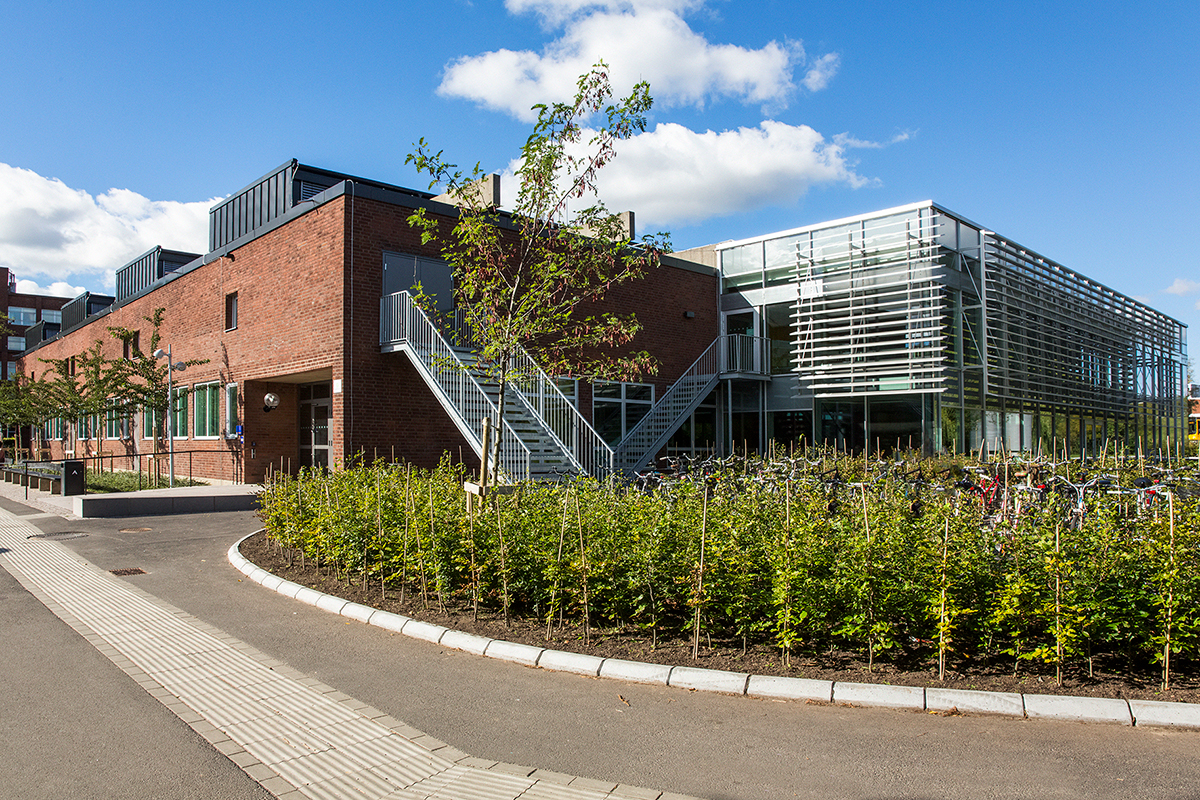
\includegraphics[height=0.41\textheight]{../img/annexet}
\end{itemize}

Besök öppna kurshemsidorna för mer information och slutna sidor i Canvas: 
\begin{itemize}
  \item \url{http://cs.lth.se/pgk} 
  \item \url{http://cs.lth.se/dod}
\end{itemize}

}


%%% AAAARGH -- version clash ? or something causing thins in Ubuntu 20.04 
%%%   but not in ubuntu 18.04:
%%%
  % ! Package pgfplots Error: Sorry, could not retrieve column 'år' from table 
  %'<inline_table>'. Please check spelling (or introduce name aliases)..

  % See the pgfplots package documentation for explanation.
  % Type  H <return>  for immediate help.
  %  ...                                              
                                                    
  % l.27 ...dplot table[x=år,y=nybörjare]{\dataSeq};

% \begin{Slide}{Andelen D-are som vid kursstart aldrig kodat}
% \pgfplotstableread[row sep=\\,col sep=&,header=true]{
%     år & nybörjare\\
%     2015 & 19  \\
%     2016 & 32  \\
%     2017 & 38  \\
%     2018 & 31  \\
%     2019 & 30  \\
%     2020 & 20  \\
% }\dataSeq

% \begin{minipage}{0.65\textwidth}
% \hspace*{-0.65cm}%
% \begin{tikzpicture}[scale=0.9, every node/.style={scale=0.9}]
%     \begin{axis}[
%             ybar,
%             bar width=1.0cm,
%             symbolic x coords={2015,2016,2017,2018,2019,2020},
%             xtick=data,
%             nodes near coords,
%             nodes near coords align={vertical},
%             legend style={at={(0.5,1)},anchor=south,legend columns=-1,draw=none},
%             ymin=0,ymax=45,
%             ylabel={\%},
%             xlabel={År},
%         ]
%         \addplot table[x=år,y=nybörjare]{\dataSeq};
%         %\legend{nybörjare}
%     \end{axis}
% \end{tikzpicture}
% \end{minipage}%
% \begin{minipage}{0.3\textwidth}
% \begin{itemize}\SlideFontTiny
% \item[] År: antal enkätsvar D
% \item[] 2015: 102 st
% \item[] 2016: 104 st
% \item[] 2017: 114 st
% \item[] 2018: 123 st
% \item[] 2019: 125 st 
% \item[] 2020: 137 st 
% \end{itemize}
% \end{minipage}%
% \end{Slide}


%%%


% \frame[plain]{\frametitle{Förkunskapsenkät}

% Ditt svar på denna \Emph{förkunskapsenkät} används i planeringen:
% \url{http://cs.lth.se/pgk/introsurvey}\\
% \Alert{Om du inte fyllt i den gör det nu!}\\
% \vspace{1em}
% Enkäten innehåller dessa frågor och några till:
% \begin{itemize}
% \item Har du programmerat tidigare? \\
%          Ja \hspace{2.5cm} Nej
% \item Hur många program har du skrivit? \\
%          $<5$ \hspace{2.2cm} $5-20$ \hspace{2.5cm}  $>20$
% \item Hur stort var det största program du har skrivit?\\
%          $<50$ rader \hspace{1cm} $50 - 500$  rader \hspace{1cm}  $>500$ rader
% \end{itemize}
% \vspace{1em}
% }

% {
%   \setbeamercolor{background canvas}{bg=black}
%   \frame{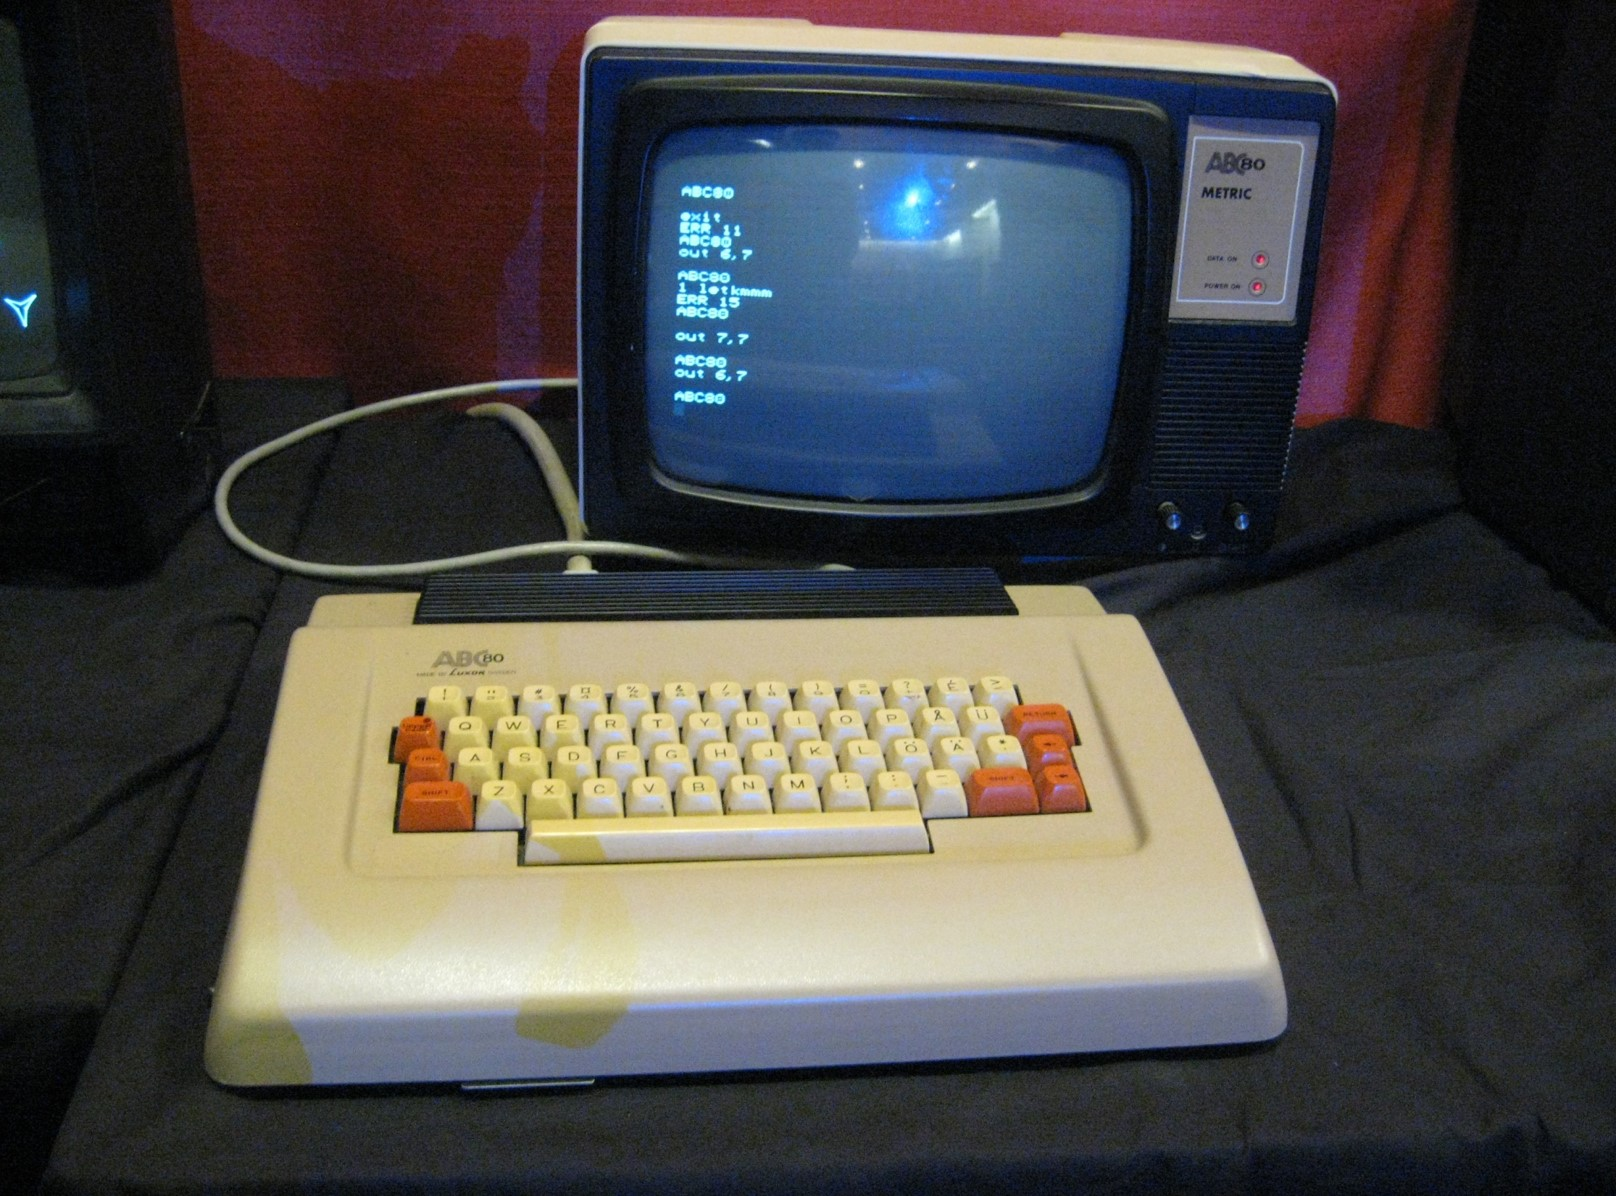
\includegraphics[width=1.0\textwidth]{../img/abc80}}
% }



\end{document}
